\documentclass{article}%You can define the type of paper here.
%%Useful packages that I commonly use.
\usepackage[numbers]{natbib}%Bibliography package (help at http://merkel.zoneo.net/Latex/natbib.php).
\usepackage{url}%Package to highlight url.
\usepackage{times}%Sets font to be times.
\usepackage{alltt}%Allows the use of verbatim (good for printing out code).
\usepackage{graphicx}%Used to import images.
\usepackage{amsmath, amssymb, amscd}%Contains the AMS expanded math symbols library.
\usepackage{algorithm, algorithmic} %pseudo-code
%%For those who want smaller margins, you can use this:
\usepackage[top=1in, bottom=1in, left=1in, right=1in]{geometry}

\begin{document}

%%Title
\title{Advanced Data Simulation and Modeling\\
       Assignment \#1}
\author{Evan Cummings}
\maketitle

%%Makes the paper use two columns
\twocolumn

%%Introduction-------------------------------------------------------------------------------------
\section{Introduction}

Our Solar System is a perfect example of a system which we can model accurately with a computer.  The model to be described herein will consist of a centrally-located fixed Sun, Jupiter, and a number of asteroids between the Sun and Jupiter.  If each planet or asteroid is given an initial tangential velocity equal to its gravitational acceleration towards the sun, stable circular orbits will form.  If the system has been created correctly, the semi-major axes of the asteroids will approach an equilibrium between the opposing forces of the Sun and Jupiter and create so-called \emph{Kirkwood Gaps} where very few asteroids reside.

Newton's law of universal gravitation provides the equations for the forces exerted between two space bodies; Kepler's laws of planetary motion provide the equations to calculate the semi-major axes of any planet's orbit around the sun. Calculating the total energy and angular momentum ensures that energy is conserved within the system and the model is performing as required.




%%Theory-------------------------------------------------------------------------------------
\section{Theoretical Equations}

% Newton :
\textbf{Newton's law of universal gravitation :}
\begin{align}
	\mathbf{F}  &= -G \frac{m_1 m_2}{r_{12}^2} \mathbf{\hat{r}}_{12} = -G \frac{m_1 m_2}{r_{12}^3} \mathbf{r}_{12},
\end{align}

where $G$ is the gravitational constant, 

$m_1$ is the mass of planet 1, 

$m_2$ is the mass of planet 2, 

${r_{12}}$ is the distance between the two planets, 

$\mathbf{\hat{r}}_{12}$ is the unit vector in the direction of planet 1 from 

planet 2, and 

$\mathbf{r}_{12}$ is the distance vector from planet 1 to planet 2.\\
\\
% Kepler :
\textbf{Kepler's third law of planetary motion :}
\begin{align}
	\frac{P_{planet}^2}{a_{planet}^3} & = 1.0 \frac{sidereal\ year^2}{AU^3},
\end{align}

where $P$ is the period of the planet and $a$ is the planet's 

semi-major axis.\\
\\
% initial tangential velocity for circular orbits :
\textbf{Initial tangential velocity for circular orbits :}
\begin{align}
	a_1 &= \frac{v_1^2}{r_{12}} = centripetal\ acceleration.\notag \\
	\implies \frac{Gm_1m_2}{r_{12}^2} &= \frac{m_1v_1^2}{r_{12}} \ using\ eq.\ (1)\ \notag \\
	\implies v_1 &= \sqrt{Gm_2 \over r_{12}}
\end{align}\\
\\
% Angular momentum :
\textbf{Angular momentum :}
\begin{align}
	\mathbf{L}=\mathbf{r}\times\mathbf{p} &= \mathbf{r}\times m \mathbf{v},
\end{align}

where $\mathbf{r}$ is the distance vector to the axis of rotation 

and $\mathbf{p} = m \mathbf{v}$ is the linear momentum vector.\\
\\
% Kinetic :
\textbf{Kinetic energy of a planet :}
\begin{align}
	K &= \frac{1}{2}m\mathbf{v}^2,
\end{align}

where $K$ is the kinetic energy of the planet, and $\mathbf{v}$ is 

its velocity vector.\\
\\
% Potential :
\textbf{Potential energy between two planets :}
\begin{align}
	U_{12} &= \frac{Gm_1m_2}{r_{12}}
\end{align}
% Total energy of a planet :
\textbf{Total energy of a planet :}
\begin{align}
	E_{tot} = K - U
\end{align}
% Total energy of a system of $n$ planets :
\textbf{Total energy of a system of $n$ planets :}
\begin{align}
	E_{sys} = &K_1 + K_2 + ... + K_n -\notag\\
	          &U_{12} - ... - U_{1n} - U_{2n}
\end{align}
% Total angular momentum of system of $n$ planets :
\textbf{Total angular momentum of system of $n$ planets :}
\begin{align}
	\mathbf{L}_{sys} = \mathbf{L}_1 + \mathbf{L}_2 + ... + \mathbf{L}_n
\end{align}
% Calculation of semi-major axis $a$ from state vectors :
\textbf{Calculation of semi-major axis $a$ from state vectors :}
\begin{align}
	a &= \frac{-\mu}{2\epsilon}\\
	\epsilon &= \frac {v^2}{2} - \frac{\mu}{|\mathbf{r}|}
\end{align}

where $\epsilon$ is the \emph{specific orbital energy},

$\mu = G(M + m)$,

$M$ is the mass of the Sun, 

$v$ is the orbital velocity of the orbiting object, and

$\mathbf{r}$ is the vector distance to the Sun.
\begin{figure}[h!]
	\centering
		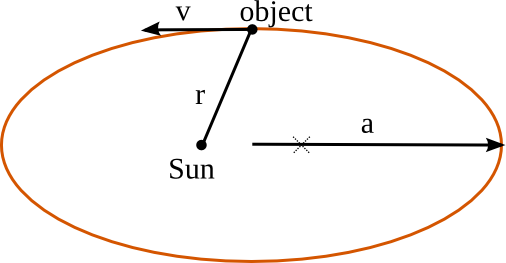
\includegraphics[width=0.35\textwidth]{images/orbits.png}
	\label{fig:orbits}
	\caption{Elliptical Orbits}
\end{figure}

%%Method-------------------------------------------------------------------------------
\section{Method}

To determine the position of a space-body after a period of time, the derivative of its position and velocity must be made. In the simplest sense :
  $$\frac {d}{dt}f(t,r) = \frac{f(t+\Delta t, r) - f(t,r)}{\Delta t}$$
  
Because the paths of the planets around the sun are elliptical, and the area swept out by a planet is constant, a method which contains an adaptive determination of the size of $\Delta t$ should be made to optimize performance.  The Dormand-Prince method of solving ordinary differential equations uses just such a method and produces a solution with a selectable error tolerance.

The position and velocity are vectors in two-dimensio-\\nal space, and as such each component must be evaluated separately :
$$\frac {d}{dt}f(t,x,y) = \frac{f(t+\Delta t, x,y) - f(t,x,y)}{\Delta t}$$

SciPy's DOPRI5 algorithm uses the Dormand-Prince method and takes as input a derivative function.  Here is pseudo-code of one implementation of just such a function with a fixed-location Sun :

\begin{algorithm}[h!]
  \caption{Calculate $\frac {d\vec v}{dt} = \vec a$ and 
                     $\frac {d\vec r}{dt} = \vec v$.}
  \begin{algorithmic} 
  \STATE \textbf{INPUTS}: 
  \STATE \ \ \ $\vec r$ - radius, $\vec v$ - velocity, $\vec m$ - mass of objects,
  \STATE \ \ \ $G$ - gravitational constant, and $M$ - mass of the sun.
  \STATE \ \ \ $t$ - time, needed for integrator
  \STATE \textbf{OUTPUTS}: 
  \STATE \ \ \ $\vec v$ - velocity, $\vec a$ - acceleration
    \FOR{$i:=0$ to $n$}
      \STATE $\vec a_i := \frac{-GM\vec r_i}{\|r_i\|^3}$
    \ENDFOR
    \FOR{$i:=0$ to $n$}
      \FOR{$j:=i+1$ to $n$}
        \STATE $\vec r_{ij} := \vec r_{j} - \vec r_{i}$
        \STATE $\vec a_i = 
               \vec a_i + \frac{Gm_j\vec r_{ij}}{\|\vec r_{ij}\|^3}$
        \STATE $\vec a_j = 
               \vec a_j - \frac{Gm_i\vec r_{ij}}{\|\vec r_{ij}\|^3}$
      \ENDFOR
    \ENDFOR
    \RETURN $\vec v, \vec a$
  \end{algorithmic}
\end{algorithm}

This function uses equation 1, and the initial velocity of each planet is found with equation 3.  DOPRI5 uses this to integrate and returns the predicted position of the planets for a given time-step, $\Delta t$.  From this a plot of positions in two-dimensional space can be made (see Figure 2).  Note also that this function can be easily converted to include the Sun as a free body by removing the first \textbf{for} loop and adding the appropriate initial values to $\vec r$, $\vec v$, and $\vec m$.

To verify that the algorithm is operating as expected, a function is needed to calculate the energy and angular momentum of the system for each time-step :

\begin{algorithm}[h!]
  \caption{Calculate energy and angular momentum.}
  \begin{algorithmic} 
  \STATE \textbf{INPUTS}: 
  \STATE \ \ \ $\vec r$ - radius, $\vec v$ - velocity, $\vec m$ - mass of objects,
  \STATE \ \ \ $G$ - gravitational constant, and $M$ - mass of the sun.
  \STATE \textbf{OUTPUTS}: 
  \STATE \ \ \ $\vec E_{tot}$ - total energy of system, 
  \STATE \ \ \ $\vec L_{tot}$ - total angular momentum of system,
  \STATE \ \ \ $\vec e$ - individual planet energy, and
  \STATE \ \ \ $\vec l$ - individual planet angular momentum.
    \FOR{$i:=0$ to $n$}
      \STATE $e_i := \frac {1}{2} m_i \|\vec v_i\|^2 - \frac{GMm_i}{\|\vec r_i\|}$
      \STATE $l_i := \vec r_i \times m \vec v_i$
    \ENDFOR
    \STATE $\vec E_{tot} := \vec e$
    \STATE $\vec L_{tot} := \vec l$
    \FOR{$i:=0$ to $n$}
      \FOR{$j:=i+1$ to $n$}
        \STATE $\vec r_{ij} := \vec r_{j} - \vec r_{i}$
        \STATE $U_{ij} = \frac{Gm_im_j}{\|\vec r_{ij}\|}$
        \STATE $e_i = e_i - U_{ij}$
        \STATE $e_j = e_j - U_{ij}$
        \STATE $E_{tot} = E_{tot} - U_{ij}$
      \ENDFOR
    \ENDFOR
    \RETURN $\vec E_{tot}, \vec L_{tot}, \vec e, \vec l$
  \end{algorithmic}
\end{algorithm}
This function uses equations 4, 5, 6, 7, 8, and 9.  The outputs can be evaluated easily by plotting the percent change at each time-step (see Figures 4 and 5).

With the output of the integrator verified, an in-depth study of the paths of asteroids can be performed.  Figure 2 displays the paths of four asteroids whose initial values of $r$ equal the semi-major axis $a$ such that the ratio $k$ of its period of revolution about the Sun to that of Jupiter is 1/2, 3/7, 2/5, and 2/3 :
\begin{align*}
  T &= \frac {2 \pi r}{v} = orbital\ period\\
  T^2 &= \frac{4 \pi^2}{GM}r^3\ by\ eq.\ (3)\\
  \implies r &= \sqrt[3]{\frac{T^2 GM}{4\pi^2}}\\
  where\ T &= k T_{Jupiter}
\end{align*}
The paths of the inner two asteroids are fairly stable, while the outer two have a more unstable "hula-hoop" like orbit around the sun (see Figure 3).

After running the simulation for a long time the values of each planet's semi-major axis $a$ will approach an equilibrium position.  Another function is needed to evaluate each planet's value for $a$ at each time-step :

\begin{algorithm}[h!]
  \caption{Calculate the semi-major axis $a$.}
  \begin{algorithmic} 
  \STATE \textbf{INPUTS}: 
  \STATE \ \ \ $\vec r$ - radius, $\vec v$ - velocity, $\vec m$ - mass of objects,
  \STATE \ \ \ $G$ - gravitational constant, $M$ - mass of the sun, and
  \STATE \ \ \ $\vec e$ - individual planet energy
  \STATE \textbf{OUTPUTS}: 
  \STATE \ \ \ $\vec a$ - semi-major axes of all planets for all $\Delta t$.
    \STATE $\vec \mu := G(M + \vec m)$
    \FOR{$i:=0$ to $n$}
      \STATE $\vec \epsilon_i := \frac{\|\vec v_i\|^2}{2} - 
                                 \frac{\vec \mu}{\|\vec r_i\|}$
      \STATE $\vec a_i := \frac{-\vec \mu}{2\vec \epsilon_i}$
    \ENDFOR
    \RETURN $\vec a$
  \end{algorithmic}
\end{algorithm}

This algorithm uses equations 10 and 11.
\textbf{NOTE:} To speed up calculations, the second outer \textbf{for} loop of Algorithm 1 can be eliminated, as the mass of each asteroid will not affect Jupiter's orbit and may be ignored.  

%%Verification-------------------------------------------------------------------------
\section{Verification of Program}
The following figures show the results of the calculations made with the algorithms described above :

\begin{figure}[H]
	\centering
		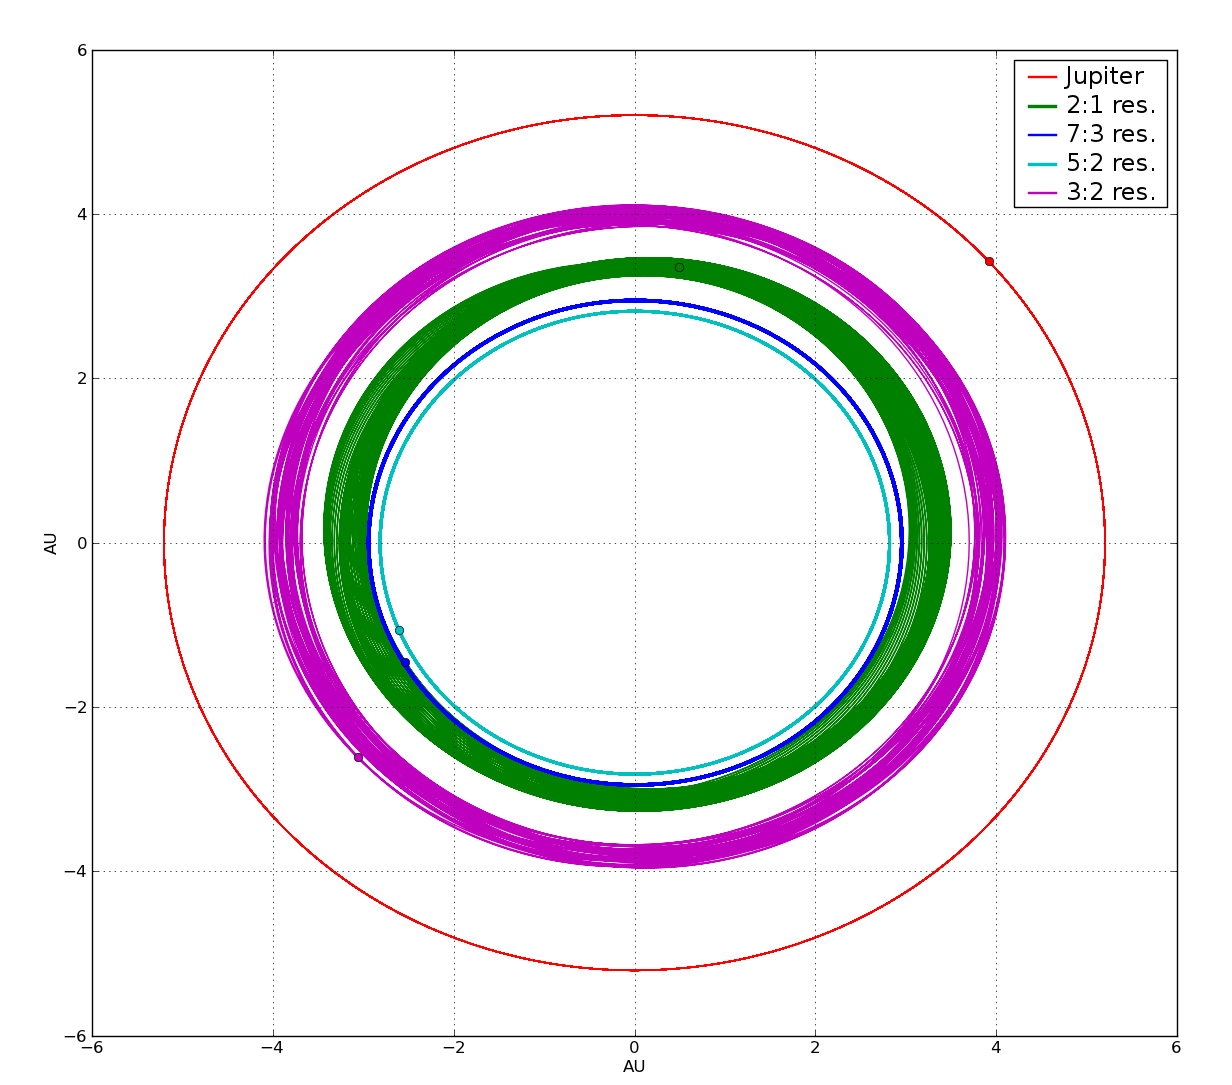
\includegraphics[width=0.50\textwidth]{images/kirkwood500yr.png}
	\label{fig:500 year orbit}
	\caption{Orbital paths of Jupiter and four asteroids around the Sun in 500 years.}
\end{figure}

\begin{figure}[H]
	\centering
		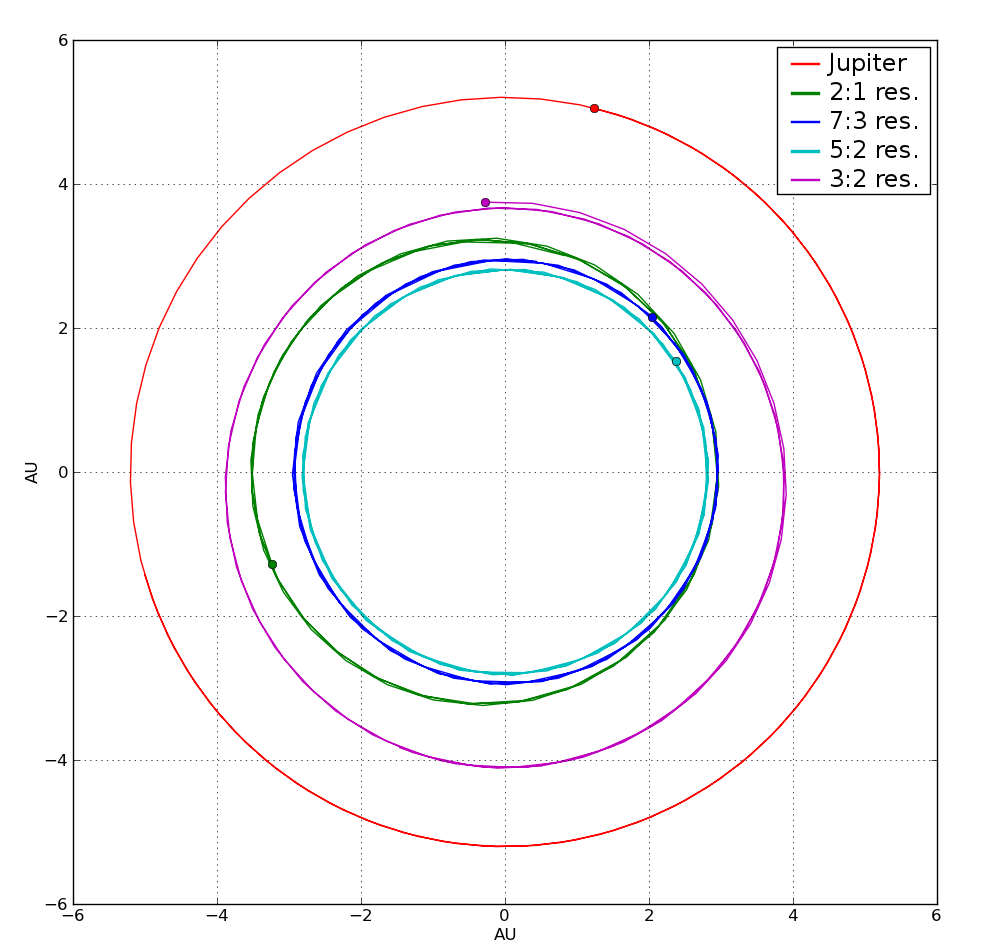
\includegraphics[width=0.50\textwidth]{images/output1000yr.png}
	\label{fig:1000 year orbit}
	\caption{Last 100 year orbit of Jupiter and four asteroids around 
	         the Sun in 1000 years.}
\end{figure}

\begin{figure}[H]
	\centering
		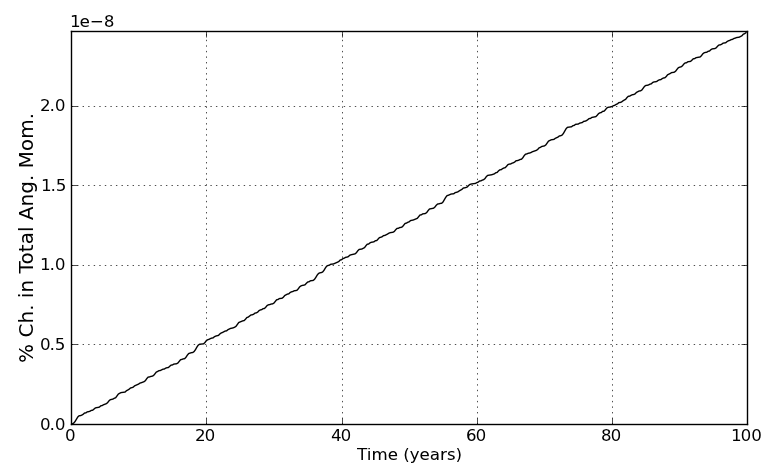
\includegraphics[width=0.45\textwidth]{images/perMom5bodies100yr.png}
	\label{fig:Change in Momentum}
	\caption{Percent change in total angular momentum for Jupiter and four asteroids  
	         in 100 years.}
\end{figure}

\begin{figure}[H]
	\centering
		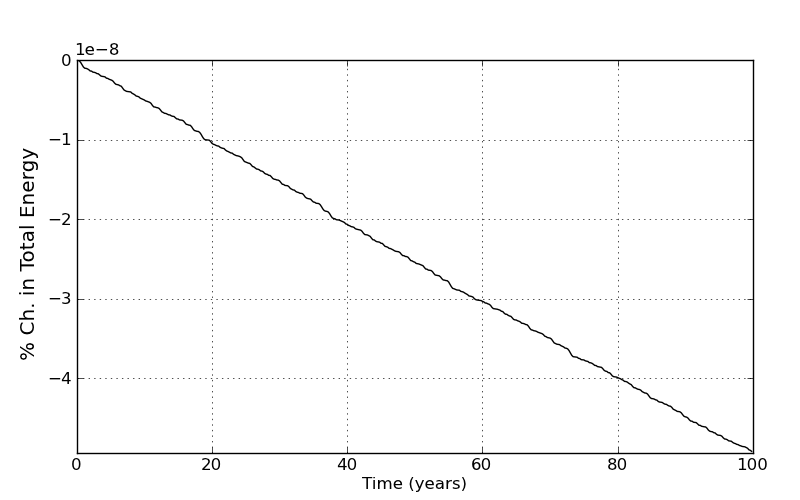
\includegraphics[width=0.45\textwidth]{images/perNrg5bodies100yr.png}
	\label{fig:Change in Energy}
	\caption{Percent change in total energy for Jupiter and four asteroids 
	         in 100 years.}
\end{figure}

\begin{figure}[H]
	\centering
		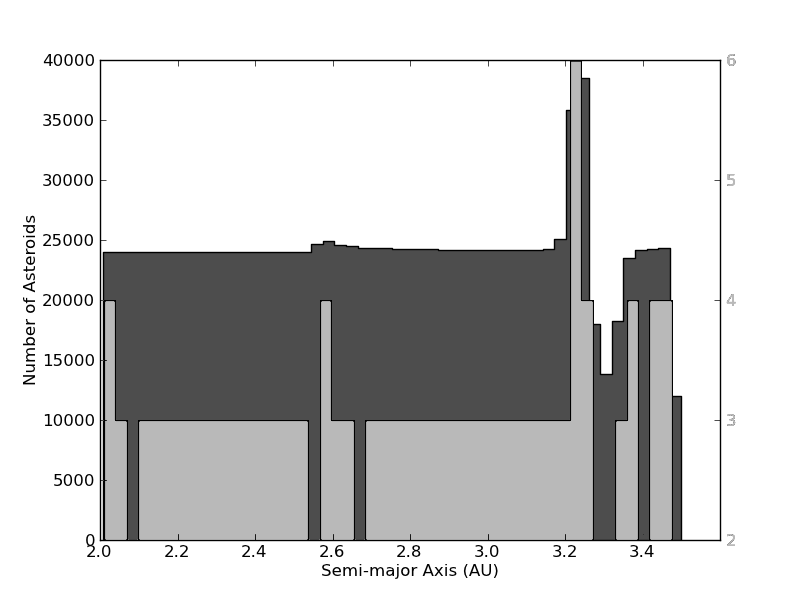
\includegraphics[width=0.50\textwidth]{images/edits/hist150ast2000yr.png}
	\label{fig:150 asteroids initial unchanged}
	\caption{Semi-major axes for 150 asteroids in 2000 years at all time-steps 
	         (dark gray) and the last time-step (light gray) with the initial 
	         velocity determined from equation 3.}
\end{figure}

\begin{figure}[H]
	\centering
		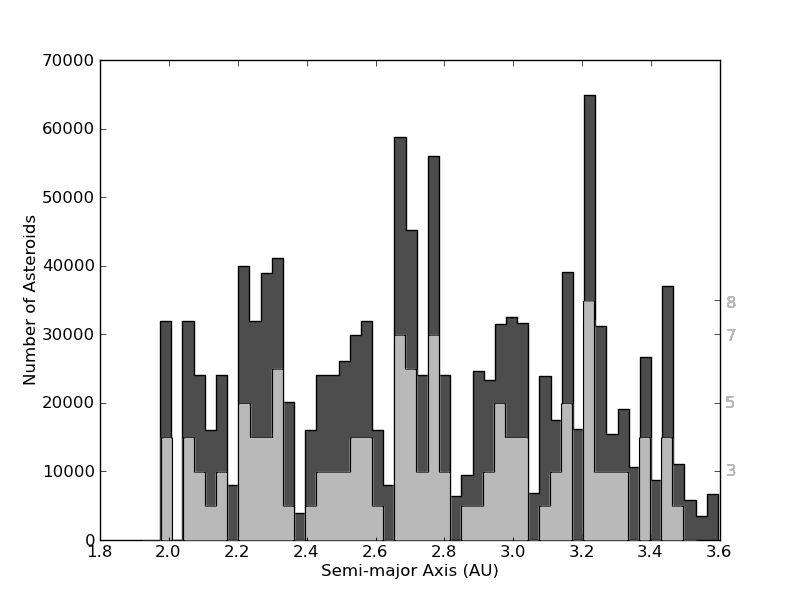
\includegraphics[width=0.50\textwidth]{images/edits/hist150ast2000yr2perRand.png}
	\label{fig:150 asteroids initial v 2perRand}
	\caption{Semi-major axes for 150 asteroids in 2000 years at all time-steps 
	         (dark gray) and the last time-step (light gray) with the initial 
	         velocity randomly determined to be $\pm$ 2\% of equation 3.}
\end{figure}

\begin{figure}[H]
	\centering
		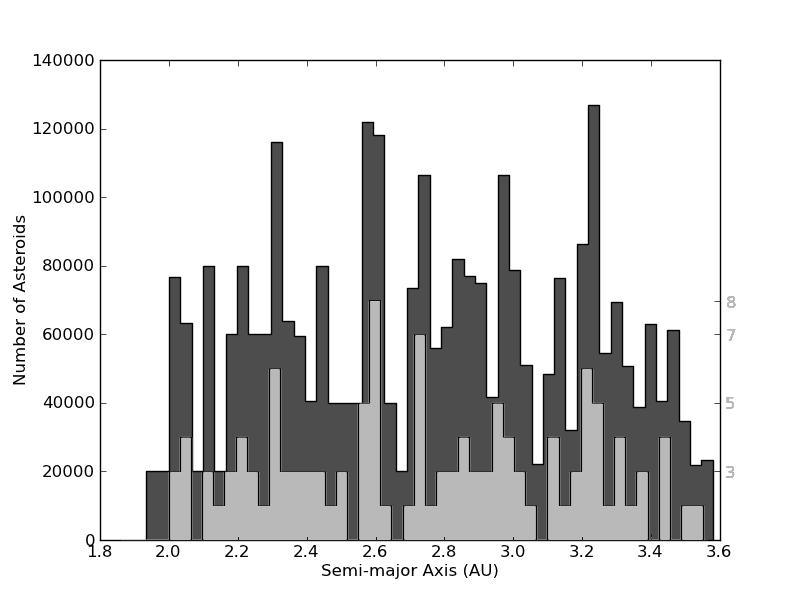
\includegraphics[width=0.50\textwidth]{images/edits/hist150ast5000yr2perRand.png}
	\label{fig:150 asteroids initial v 2perRand}
	\caption{Semi-major axes for 150 asteroids in 5000 years at all time-steps 
	         (dark gray) and the last time-step (light gray) with the initial 
	         velocity randomly determined to be $\pm$ 2\% of equation 3.}
\end{figure}

\begin{figure}[H]
	\centering
		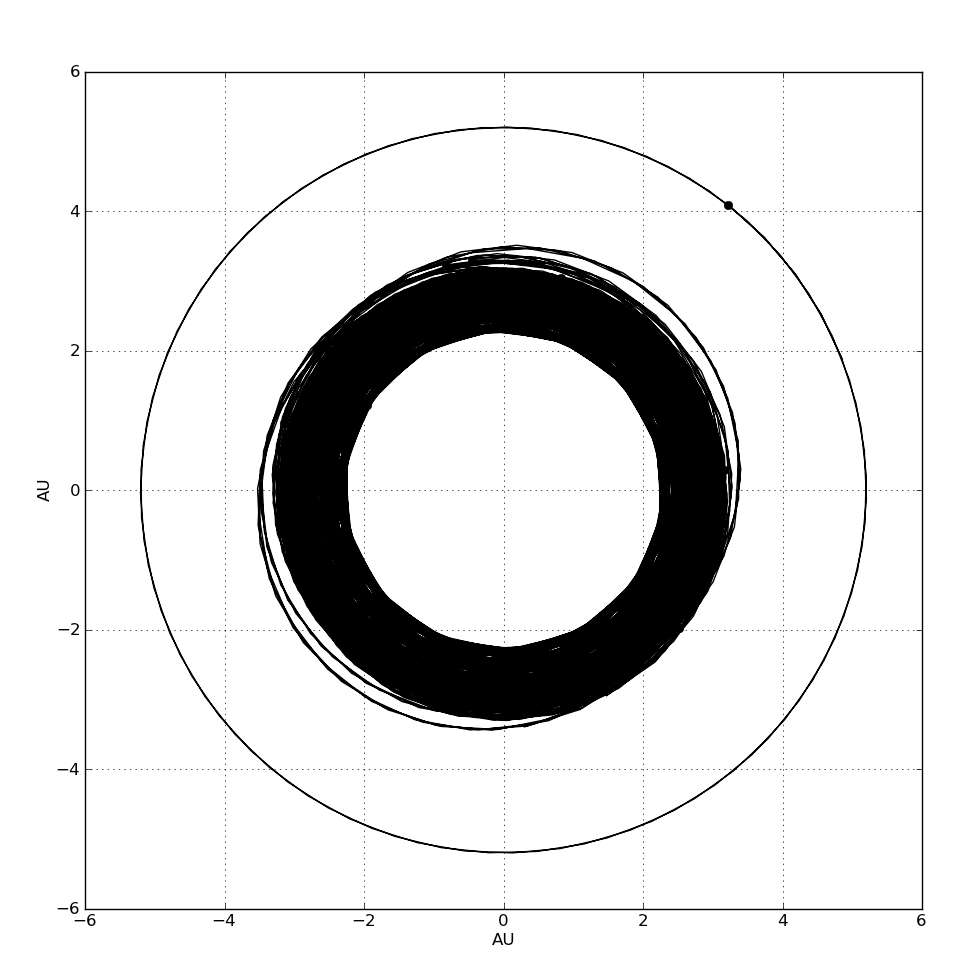
\includegraphics[width=0.50\textwidth]{images/edits/output100ast5000yr.png}
	\label{fig:150 asteroid orbits}
	\caption{Final 100 years of 150 asteroid paths after 5000 years with an initial 
	         velocity randomly determined to be $\pm$ 2\% of equation 3.}
\end{figure}
\onecolumn
\twocolumn

%%Interpretation------------------------------------------------------------------
\section{Interpretation}

Figures 2 and 3 show four asteroids initially placed at the 2:1 resonance at 3.27 AU, 7:3 resonance at 2.95 AU, 5:2 resonance at 2.82 AU, and 3:2 resonance at 3.97 AU. The 7:3 and 5:2 resonance asteroids do not show as much variation as would be expected, but their relatively close proximity to the Sun may make it take longer for Jupiter to have an effect on their orbits.

Creating 150 asteroids equally spaced within 2.0 and 3.5 AU of the sun produce interesting results (see figures 6, 7, 8, and 9).  The data also show that with a randomly determined initial value of $v$, the semi-major axis of an asteroid placed between the Sun and Jupiter approach an equilibrium, and in all histograms the last values quite closely match the entire set.  Changing DOPRI5's \emph{atol} and \emph{rtol} tolerance values reduce the percent change in energy and angular momentum, but produce little change on the gap locations.  Although different runs do not contain gaps in identical locations, I hypothesize that with enough iterations there would be voids located similarly to the real \emph{Kirkwood Gaps}.

%%Bibliography--------------------------------------------------------------------
\begin{thebibliography}{1}
	\bibitem{1}Gould, H., Tobochnik, J., \& Christian, W. (2007). \textit{An Introduction to Computer Simulation Methods: Applications to Physical Systems}. San Francisco, CA: Pearson Education, Inc.
\end{thebibliography} 

\end{document}
%%Compile with pdflatex file.tex

